
\chapter{Static Analysis \label{chapter:analysis}}

In this chapter, we will introduce concept of static analysis,
its possible applications and its limitations,
focusing especially on aspects relevant for computing data lineage.



\section{Program Analysis}

\textbf{Program analysis} is the process of automatically analyzing the behavior
of computer programs. There are two principal approaches to such analysis:
\begin{itemize}
  \item \textbf{Dynamic program analysis} is performed during program runtime.
    To perform dynamic analysis, both executable program
    and its inputs are required. To be effective, the target program
    must be executed with sufficient test inputs, as its results
    are limited only to observed executions of the analyzed program.
  \item \textbf{Static program analysis} is the program analysis that is actually
    performed without executing the input program. The analysis is usually
    performed on the intermediate representation (IR) of the program source code
    (used e.g. in compilers), or bytecode.
    Results of static program analysis cover all execution paths of
    analysed program.

    Static program analysis technique is very popular. It is thanks
    to its speed, reliability and sometimes it is the only possible
    way for complex systems in reasonable time.
    It is often used to detect program errors, such as
    security vulnerabilities or performance issues.
\end{itemize}

\textbf{Data flow analysis} is a technique for gathering information about
all possible values of variables during program execution.



\section{WALA Framework \label{chapter:analysis:wala}}

The T. J. Watson Libraries for Analysis, the \citet{WalaFramework},
is a framework for static analysis capabilities for Java
bytecode and related languages.

The main goals of WALA Framework are:
\begin{itemize}
  \item Robustness
  \item Efficiency
  \item Extensibility
\end{itemize}

The key features WALA Framework provides are:
\begin{itemize}
  \item Pointer analysis
  \item Class hierarchy
  \item Call graph
  \item Interprocedural dataflow analysis
  \item Context-sensitive slicing
\end{itemize}

We describe some of the features in the following subsections.



\subsection{Pointer analysis}

\citet{PointerAnalysis} define \textbf{pointer analysis},
or \textbf{points-to analysis} respectively, as a static program analysis that
determines information on the values of pointer variables or expressions.
It is near-synonym of \textbf{alias analysis} that use \citet{AliasAnalysis}.
Pointer analysis typically answer question
\uvodzovky{what objects can a variable point to?},
whereas alias analysis focus on closely related question
\uvodzovky{can a pair of variables point to the same object?}.




\subsubsection{Flow and Context Sensitivity}

Flow sensitivity refers to ability of an analysis to take control flow
into account when analyzing a program.
In case, analysis considers statement ordering, it is called \textbf{flow-sensitive},
otherwise it is \textbf{flow-insensitive} analysis.

Contex sensitivity can be taken into account in an interprocedural analysis and
then we call it \textbf{contex-sensitive}. Otherwise, when calling context is ommited,
such an analysis is called \textbf{context-insensitive}.




\subsection{Class hierarchy}

A \textbf{class hierarchy} is a structure for set of classes
of the analyzed program. It includes also information about the used
programming language and the relationships between such classes.

Such relations in programs written in Java language are the \Code{implements} and \Code{extends}
relations.

Each class also includes collection of its methods. Methods can be declared in the
class, or inherited from parent.



\subsection{Call Graph}

A \textbf{call graph} represents calling relationships between subroutines
in an analysed computer program. The nodes represents procedures and each
directed edge represents procedure calls.

When used in context-sensitive manner, it means that for each procedure 
the graph contains a separate node for each call stack that procedure can be
activated with.




\section{Symbolic Analysis Library \label{chapter:analysis:symbolicAnalysisLibrary}}

\textbf{Symbolic analysis library} is a library for computing flow of information
in Java program - the data lineage.
The Symbolic analysis library is based on symbolic Java bytecode interpreter
that was introduced in \citet{ParizekHybridAnalysis}
and used in the ongoing whose results will be published
in a short time in \citet{ParizekBUBEN}.

The library uses static analysis techniques to construct call graph and
for each method it computes its summary for different invocation contexts (symbolic parameter values)
based on symbolic bytecode interpretation.

The bytecode analysis is done using \citet{WalaFramework}
that was described in Section \ref{chapter:analysis:wala}.

Bytecode interpreter performs linear traversal of the method bytecode instructions
and computes various information for symbolic variables and constant expressions.

The Symbolic analysis library creates method summaries that for each
local variable (fields, arrays or complex expression) contains
data sources and the concrete values (for \Code{String}s and numbers).



\subsection{Symbolic Analysis Algorithm}

The symbolic analysis algorithm for computing static method summaries use:
\begin{enumerate}
  \item A \textbf{fixpoint worklist algorithm} over the list of all reachable methods.
  \item A \textbf{linear symbolic interpretation} of the bytecode of methods.
\end{enumerate}

The library is iteratively updating its method summaries until the fixpoint is reached, i.e.
when summaries are not changing.

Several method invocation contexts (method parameters with their associated data flow information)
are distinguished. When the newly computed summary for a given method is different from the previous
one, all callers and calles of the method are added to the worklist in order to achieve soundness.
The algorithm terminates when the summary of each method captures all its results and side effects.




\subsection{Flow Propagation}

In the previous section we described general algorithm for symbolic analysis.
However, we did not specify, how the flow information is used in practice.

Now we describe selected important aspects and features of the Symbolic analysis library
that are relevant for data lineage information.




\subsubsection{Library Methods}

As optimizations, library does not process all reachable methods.
It analyses just methods of application code and procedures with special
meaning that are described in next sections.

For ignored methods, the \textbf{identity} is returned.
The identity function with respect to flow data propagation is defined as
merge of flow data of receiver (the object on which method is called) and
all arguments of that method. The result of that merge is then associated
as flow data of returned value and receiver.




\subsubsection{Strings}

Knowing the concrete values of the \Code{String} used in application is valuable
when it comes to data lineage of application.
\Code{String}s identify file names that are accessed in application,
or it can be SQL query to database, etc.

However, concrete values are known only when using as literal in the application.
Sometimes, the symbolic analysis cannot determine the precise concrete string value.
It is often when it is loaded from file or database, or after some operations
like \Code{trim}, \Code{substring}, or even concatenation of \Code{String}s
(which works only for \Code{String} literals).
Then the actual value is in general unknown, but the flow information must be preserved.




\subsubsection{Numeric types}

Handling concrete values for numeric Java types works as in case
of \Code{String} literals. It is useful to know them, but often
they cannot be determined. Flow information must be preserved after
the operations with the numbers in any case.




\subsubsection{Arrays and Collections}

Arrays and collections are integral parts of Java. In this part we describe how
they are handled in propagation of flow.

The basic approach is not to distinguish individual items and use just one
abstract element summary. In that case, as over-approximation, all possible elements
of a given array or collection are considered.
Complete flow information is also used when creating \Code{java.util.Iterator}
from a collection.

Also, when using \Code{java.util.Map} and \Code{java.util.Properties} instances,
analysis does distinguish the keys and corresponding values.
and 
analysis does not distinguish between used keys and corresponding values
and maintains just a single set of flow for the whole class.

In case of collections of \Code{String}s or numeric values, library provides
the information about concrete values stored in collections whenever possible.





\subsection{Identifying the Sources and Sinks of a Data}

Symbolic analysis algorithm that we describe in previous section is
used to compute data flow in application.
When such sources or sinks are identified, the algorithm would
propagate such data flow.

Now, the problem is to identify the sources and sinks of a data
in the application.




\subsubsection{Java IO}

Java input and output (IO) operations can be used to access data in application.
It can be done through standard application
\Code{System.in}, \Code{System.out} and \Code{System.err},
where they are identified by the name \uvodzovky{System.in}, etc.
or using external files, where its file name identifies the source (or sink respectively).

The library handles both cases and correctly identifies
all the read and write operations of such inputs and outputs.

The library focuses only to inputs and outpus made by classes in \Code{java.io} package
but also the \Code{java.nio} package would be supported soon.




\subsubsection{JDBC API}

The library also contains implementation for identification of
database reads and writes using plain JDBC API.
The related usage of the JDBC API was already described in Section \ref{frameworks:jdbc}.

The library can identify the connection url for the database
that application is connecting to, SQL queries and the columns
that are read from results in \Code{ResultSet}.

The library focuses only on classes in the package \Code{java.sql}
therefore \Code{javax.sql} API is not supported.



\subsubsection{Extendability}

The symbolic analysis library can be extended to support other types
of data sources and sinks. We will describe this feature in the section \ref{chapter:implementation:interface}.



\subsection{Data Lineage Visualization \label{chapter:analysis:visualization}}

The data flow graph is created based on the results of symbolic analysis - based on
the computed method summaries.

The graph nodes consist of a set of identified sources and sinks for the data
and its oriented edges are between pair of nodes between which the data flows.

The graph visualization is then created using \citet{Graphviz} tool in resulted PDF file.
The structure of the graph is described in more detail in section \ref{chapter:program:graphs}.

There are more types of graph nodes, from which the most important are:
\begin{itemize}
  \item \Code{Connection} - defines JDBC connection to database.
  \item \Code{SQLCommand} - defines standard JDBC SQL query.
  \item \Code{StreamAction} - defines action on stream (files IO, standard IO).
  \item \Code{EntryArgument} and \Code{EntryArgumentData} - defines data flow from entry arguments.
  \item \Code{EntryReturnVal} and \Code{EntryReturnValData} - defines data flow to entry method result.
\end{itemize}

Each node contains few attributes that describes the location where an operation was made
(\Code{java\_class\_desc} and \Code{java\_method\_desc} identifies the Java class and method, where operation was made)
and more information about the data lineage for such operation.
For example, \Code{Connection} node contains connection url in \Code{db\_connection\_desc}
attribute and the user used to connect to database is in \Code{db\_connection\_user\_desc}.
Other example can be the \Code{SQLCommand} node with the SQL statement in attribute \Code{db\_statement\_desc},
or \Code{stream\_location\_desc} identifies the name of used file in \Code{StreamAction} node,
or standard input and outputs (\Code{System.in}, etc.).

The entry nodes (\Code{EntryArgument}, \Code{EntryReturnVal}, etc.) show that data can flow
into analysed method as its argument, or flow out from a method as its result.

Listing \ref{code:dbio} show more complex example, where both database and file
operations occurs. For simplicity we omit boilerplate code (such as closing connections and file stream, etc.).

On line \ref{code:dbio:connection}, the database connection is opened,
on lines \ref{code:dbio:statement:begin}--\ref{code:dbio:execute} the query
with \Code{id} argument is created and executed. From \Code{ResultSet} the \Code{VALUE}
column is loaded and on line \ref{code:dbio:writeFile} its value is written to the file \Code{outputFile.txt}.

\InsertCode{h}{code/dbio.tex}

Figure \ref{frameworks:dbio:graph} contains visualization of the data flow graph
of the \Code{writeValue\-ForIdToFile} method from Listing \ref{code:dbio}.
We just omit some unessential information from nodes.

The visualization contains following nodes:
\begin{enumerate}
  \item \Code{EntryArgument0} and \Code{EntryArgumentData0} nodes for identification of \Code{id} argument.
  \item \Code{Connection} node for identification of database connection - url and user.
  \item \Code{ParamIndex} and \Code{SQLCommand} nodes for identification of database query.
  \item \Code{ResultColumn} node for loading value from a query.
  \item \Code{StreamAction} nodes for identification of output file.
\end{enumerate}

Besides the main flow in the graph from database query to output file, we can
notice that correct file name (\Code{outputFile.txt}) is computed by the library.
Notice also flow from \Code{id} argument into SQL statement as its parameter.

In the visualization we can also notice two \Code{StreamAction} nodes but with different
tags - \textit{Open} and \textit{Write}.
Tags represents the operations that were made to that stream. The flow
goes from \textit{Write} to \textit{Open}, as the \Code{write} call is made on the opened stream.

\begin{figure}[p]
  % trim - left lower right upper
  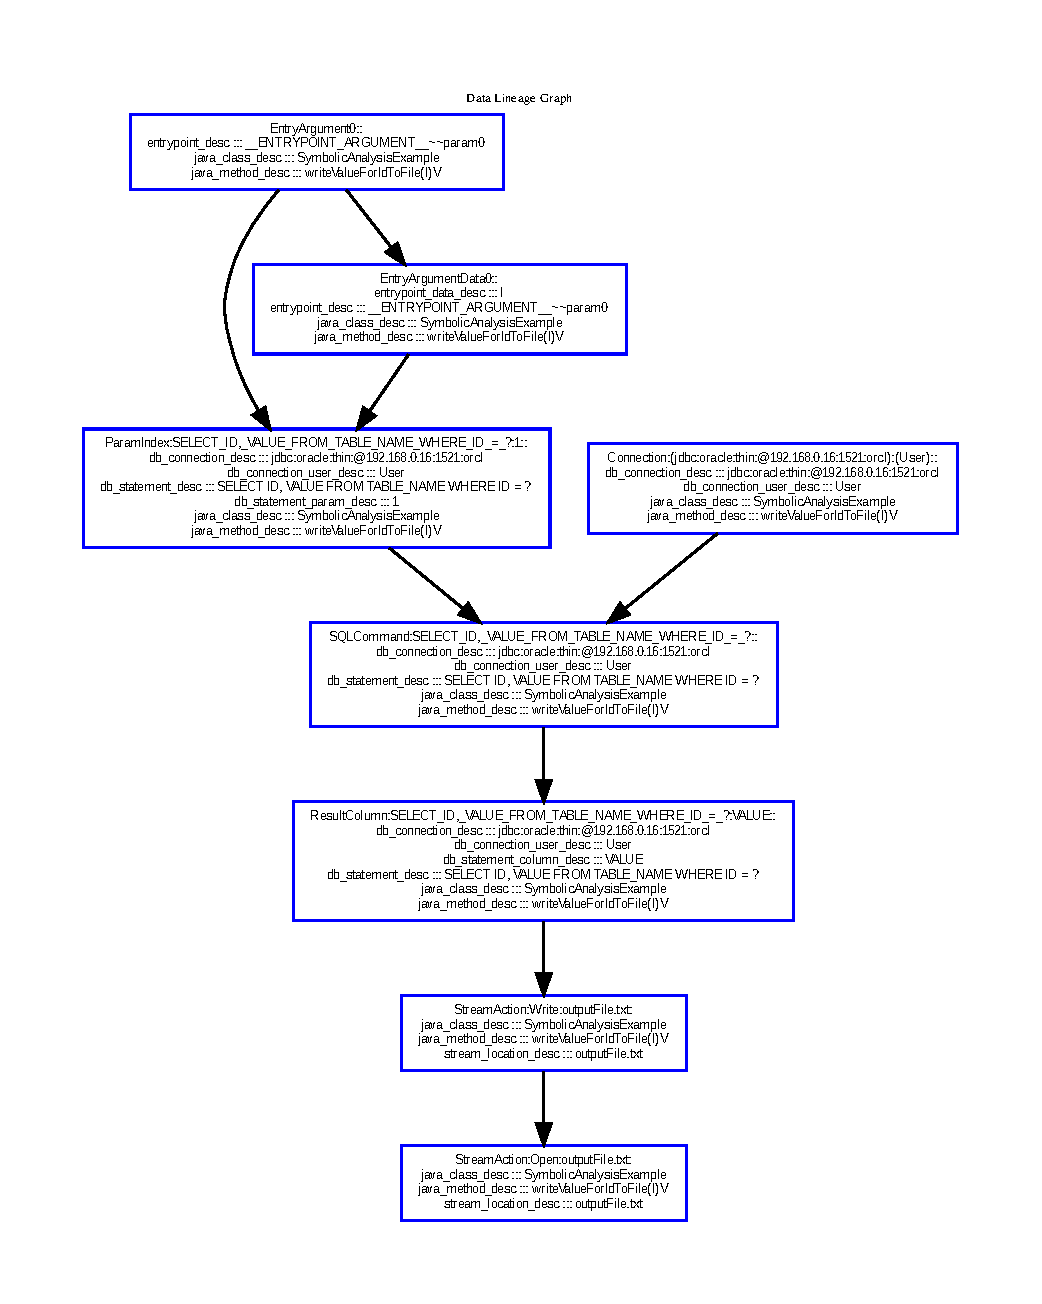
\includegraphics[trim={1cm 1cm 1cm 1.8cm},clip,width=\textwidth]{img/Examples2-writeValueForIdToFile.pdf}
  \caption{Visualization of data lineage graph}
  \label{frameworks:dbio:graph}
  \hspace{-15mm}
\end{figure}

